\section{Supplementary figures and tables}
\begin{table}[H]
\centering\renewcommand\cellalign{lc}
\setcellgapes{3pt}\makegapedcells
\begin{tabular}{|l|l|} \hline
  \makecell{Number of unique news stories} &$88,316,898$\\ 
  \makecell{Number of stories remaining after removing topics including\\ analyst recommendations, ratings changes, and index movements}&$87,841,641$\\
  \hspace{3mm}Of these: &\\
  \hspace{3mm}Number of stories tag sample companies& $8,341,848 $\\
  \hspace{5mm}Of these: &\\
  \hspace{5mm}Number of stories that mention only one company& $5,507,772 \hspace{1mm}(66.03\%)$\\
  \hspace{5mm}Number of stories that mention exactly two companies& $1,637,256 \hspace{1mm}(19.63\%) $ \\
  \hspace{5mm}Number of stories that mention more than two companies&$1,196,820 \hspace{1mm}(14.34\%)$ \\
\hline\end{tabular}
\caption{Descriptive statistics for RavenPack Equity files Dow Jones Edition for the period January 2004 to December 2015.}
\label{table:news}
\end{table}


\begin{table}[H]
    \centering
  \begin{tabular}{cccc}
  \hline
  Number of yearly window a pair gets identified& Frequency & Percentage& Cumulative Percentage\\
0   & 217024&      $72.80\%$ & $72.80\%$\\ 
1 &          40178   &   $13.48\%$ & $86.28\%$ \\ 
2     &      13302 &     $4.46\%$ & $90.74\%$\\ 
3         &  7116    &  $2.39\%$ & $93.13\%$\\ 
4      &     4522   &   $1.52\%$ & $94.65\%$\\ 
5        &   3236     & $1.09\%$ & $95.74\%$\\ 
6       &    2506    &$0.84\%$ & $96.58\%$\\ 
7        &   2022    & $0.68\%$ & $97.26\%$\\ 
8         &  1804   &  $0.61\%$ & $97.87\%$\\ 
9          & 1508   &  $0.51\%$ & $98.38\%$\\ 
10          & 1350    & $0.45\%$ & $98.83\%$\\ 
11           &1232     &$0.41\%$ & $99.24\%$\\ 
12           &2316     & $0.78\%$& $100\%$\\ 
\hline
\end{tabular}
\caption{Frequency distribution table of the number of yearly link identification windows that a pair gets identified as economic neighbors for all possible pairs $(i,j)$ in our sample. Note: A pair identified in $k$ yearly windows could get multiple co-mentions within each window. }
\label{table:freq}
\end{table}


\begin{figure}[H]
    \centering
    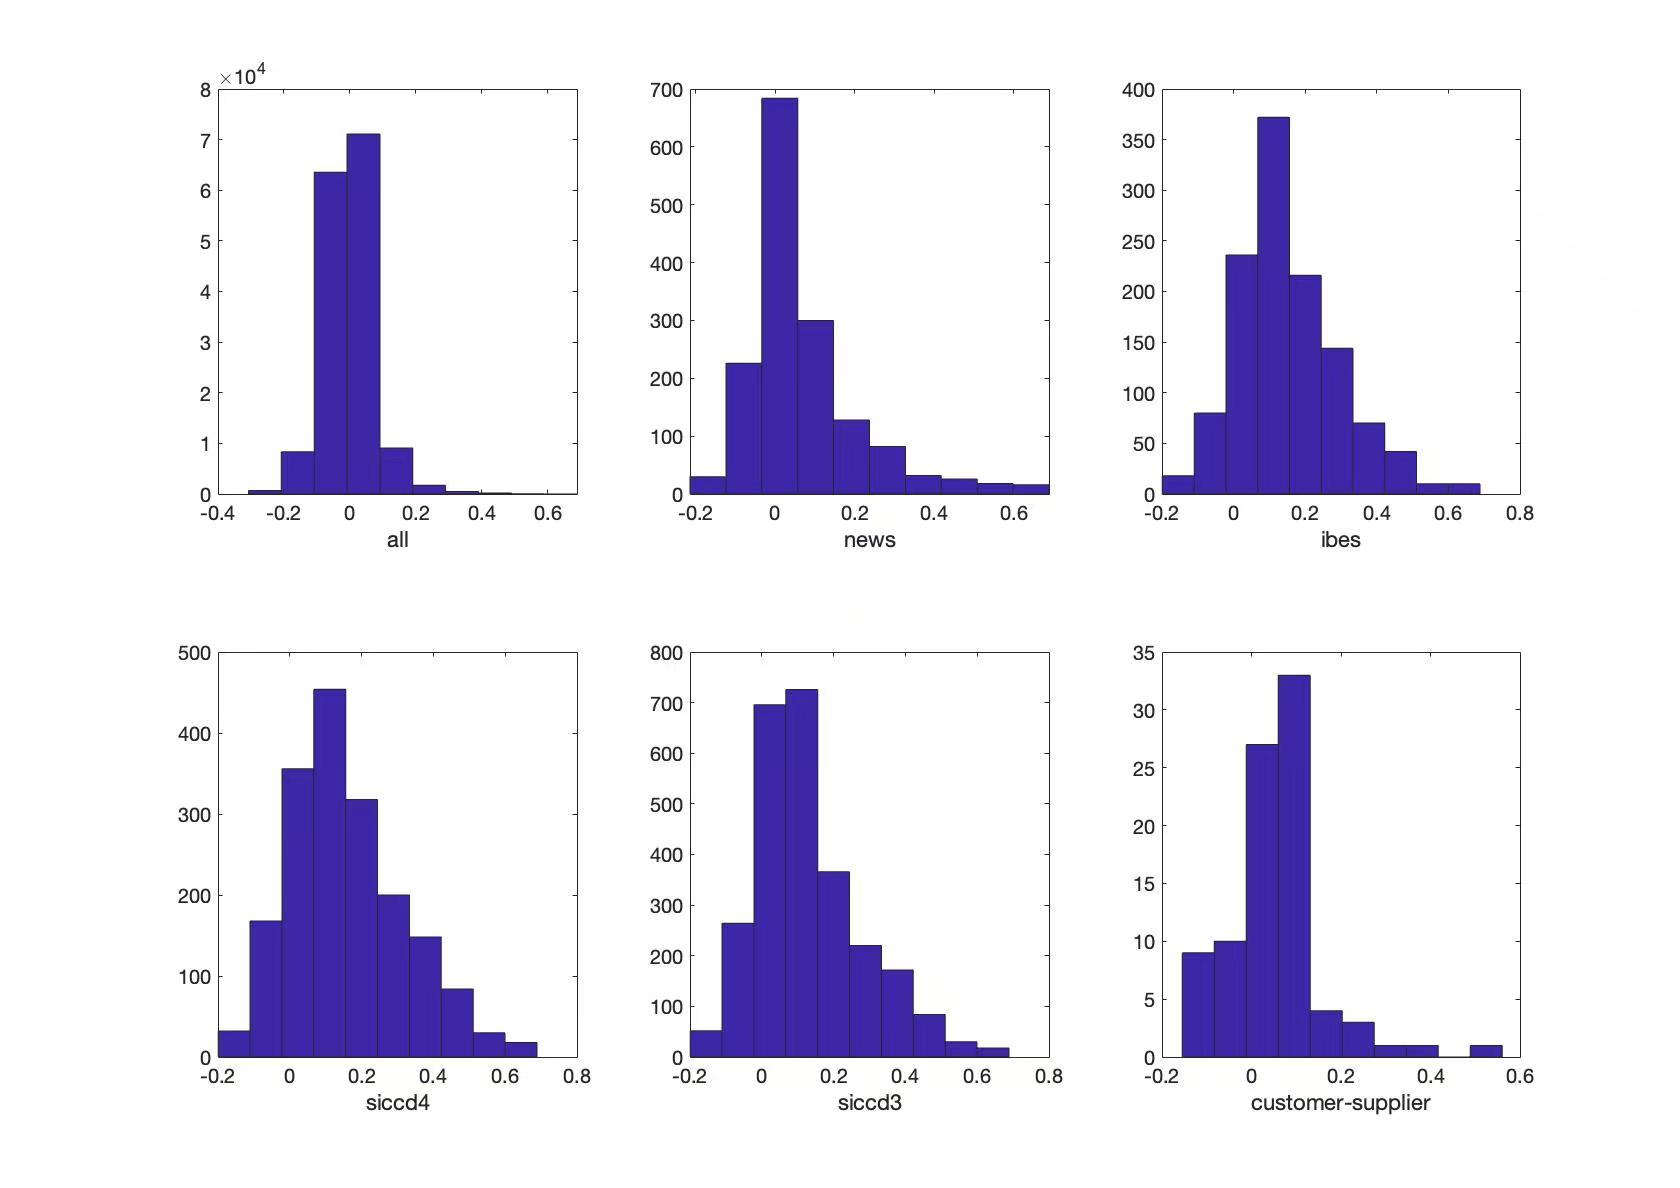
\includegraphics[scale=0.25]{pic/corr_5pca.jpg}
    \caption{Histograms of factor model residual correlations. Correlations are calculated on the residuals after removing five principal components. The top left sub-figure shows the histogram of all non-diagonal residual correlations. The rest sub-figures show the histograms of residual correlations among linked pairs.}
    \label{fig:corr5_pca}
\end{figure}


\section{Proof of Theorem 1}
\begin{proof}{ of Theorem \ref{theorem1}}

    Suppose \(F\) is Gaussian and for sufficiently large \(M\), 
    \begin{equation*}
            \lambda = M \sqrt{\frac{\log N}{T}}
    \end{equation*}
    and \(\frac{\log N}{T} \to 0\) as \(T \to \infty\), 
    then for the operator norm \(\norm{M}= \max_{j} \abs{\lambda_{j}(M)}\) where \(\lambda_{1},\dots,\lambda_{N}\) are the eigenvalues of \(M\), \autoref{theorem1} establishes that
        \begin{equation*}
      \norm{T_{\hat{L},\lambda}\pqty{\hat{\Sigma}} - \Sigma } = O_{p}\pqty{c_{1}(p) \sqrt{\frac{\log N}{T}}+c_{0}(p)\pqty{\frac{\log N}{T}}^{\frac{1-q}{2}}}
       \end{equation*}
    Consider the following decomposition:
    \begin{equation*}
        \norm{T_{\hat{L},\lambda}\pqty{\hat{\Sigma}} - \Sigma } \leq \norm{T_{\hat{L} ,\lambda}(\Sigma) - \Sigma} +\norm{T_{\hat{L}, \lambda}(\hat{\Sigma}) - T_{\hat{L},\lambda}(\Sigma)} = \mathbf{I} + \mathbf{II}
    \end{equation*}
    The first term can be bounded by 
    \begin{align*}
        \mathbf{I} &\leq \max_{i} \sum_{j} \abs{s_{\hat{L}, \lambda}(\sigma_{ij}) - \sigma_{ij}} \\
        &= \max_{i} \sum_{j} \hat{L}_{ij}^{0} \abs{s_{\lambda}(\sigma_{ij}) - \sigma_{ij}}\\
        &= \max_{i} \sum_{j} \bqty{L_{ij}^{0} \abs{s_{\lambda}(\sigma_{ij}) - \sigma_{ij}} + (\hat{L}_{ij}^{0} - L_{ij}^{0})\abs{s_{\lambda}(\sigma_{ij}) - \sigma_{ij}}} \\
        &\leq (1 + o_{p}(1))\max_{i} \sum_{j} \bqty{L_{ij}^{0} \abs{s_{\lambda}(\sigma_{ij}) - \sigma_{ij}}}\\
        &\leq (1 + o_{p}(1))\max_{i} \sum_{j} \bqty{L_{ij}^{0} \abs{\sigma_{ij} \mathbf{1}\Bqty{\sigma_{ij}\leq \lambda} + (s_{\lambda}(\sigma_{ij}) - \sigma_{ij}) \mathbf{1}\Bqty{\sigma_{ij} > \lambda}}}\\
        &\leq (1 + o_{p}(1)) \max_{i} \sum_{j} \bqty{L_{ij}^{0}\abs{\sigma_{ij}}^{q} \lambda^{1 -q}}\\
        &\leq (1 + o_{p}(1)) c_{0}(p) \lambda^{1-q}
    \end{align*}
    And the second term can be bounded similar to \cite{rothman2009generalized}, 
    \begin{align*}
        \mathbf{II} &\leq  \max_{i} \sum_{j} \bqty{\hat{L}_{ij}^{1} \abs{\hat{\sigma}_{ij} - \sigma_{ij}} + \hat{L}_{ij}^{0} \abs{s_{\lambda}(\hat{\sigma}_{ij}) - s_{\lambda} (\sigma)_{ij}}}\\
        &\leq (1 + o_{p}(1))c_{1}(p)\max_{ij} \abs{\hat{\sigma}_{ij} - \sigma_{ij}} + (1 + o_{p}(1)) \max_{i} \sum_{j} L_{ij}^{0} \abs{s_{\lambda}(\hat{\sigma}_{ij}) - s_{\lambda} (\sigma)_{ij}} \\
        &= O_{p}\pqty{c_{1}(p) \sqrt{\frac{\log N}{T}} + c_{0}(p) \pqty{\lambda^{1-q} + \lambda^{-q} \sqrt{\frac{\log N}{T}}}} \\
    \end{align*}
    Hence we have 
    \begin{align*}
        \norm{T_{\hat{L},\lambda}\pqty{\hat{\Sigma}} - \Sigma } &= O_{p}\pqty{c_{1}(p) \sqrt{\frac{\log N}{T}} + c_{0}(p) \pqty{\lambda^{1-q} + \lambda^{-q} \sqrt{\frac{\log N}{T}}}} \\
        &= O_{p}\pqty{c_{1}(p) \sqrt{\frac{\log N}{T}} + c_{0}(p)\pqty{\frac{\log N}{T}}^{\frac{1-q}{2}}}
    \end{align*}
\end{proof}


\section{Proof of Theorem 2 and 3}
\begin{lemma}
    For a series $\{ a_n \geq 0 \}$, denote $a_{(i)}$ as the $i$-th largest element. If $\sum_{i=k+1}^\infty a_{(i)} = O(k^{-\alpha})$, then $a_{(k)} = O(k^{-\alpha-1})$.
    \label{lemma_sum_single}
\end{lemma}

\begin{lemma}
    If $X_n = O_P(Y_n)$ and $Y_n = O_P(a_n)$, then $X_n = O_P(a_n)$. If $X_n = O_P(a_n)$ and $Y_n = O_P(b_n)$, then $X_n Y_n = O_P(a_n b_n)$.
    \label{lemma_OP}
\end{lemma}

\begin{proof}{ of Lemma \ref{lemma_OP}}

    (1)
    $\forall \epsilon, \exists M_1(\epsilon), N_1(\epsilon), \forall n > N_1, \Pr \{ |X_n/Y_n| > M_1 \} < \epsilon $. Similarly, $M_2(\epsilon)$ and $N_2(\epsilon)$ for $Y_n = O_P(a_n)$. If we choose $M = \max\{ M_1^2(\frac{\epsilon}{2}), M_2^2(\frac{\epsilon}{2}) \}$ and $N = \max \{ N_1(\frac{\epsilon}{2}), N_2(\frac{\epsilon}{2}) \}$, then $\forall n > N(\epsilon)$ we have 
    \begin{equation}
        \begin{split}
            \Pr \{ |\frac{X_n}{a_n}| > M \} &= \Pr\{ |\frac{X_n}{Y_n}| > \sqrt{M} \ \land \ |\frac{X_n}{a_n}| > M \} + \Pr \{ |\frac{X_n}{Y_n}| \leq \sqrt{M} \ \land \ |\frac{X_n}{a_n}| > M \} \\
            &\leq \Pr \{ |\frac{X_n}{Y_n}| > \sqrt{M} \} + \Pr \{ |\frac{Y_n}{a_n}| > \sqrt{M} \} \\
            &< \epsilon
        \end{split}
    \end{equation}

    (2)
    $\forall \epsilon, \exists M_1(\epsilon), N_1(\epsilon), \forall n>N_1, \Pr \{ |X_n/a_n| > M_1 \} < \epsilon $. Similarly, $M_2(\epsilon)$ and $N_2(\epsilon)$ for $Y_n = O_P(b_n)$. If we choose $M = \max\{ M_1^2(\frac{\epsilon}{2}), M_2^2(\frac{\epsilon}{2}) \}$ and $N = \max \{ N_1(\frac{\epsilon}{2}), N_2(\frac{\epsilon}{2}) \}$, then $\forall n>N(\epsilon)$ we have
    \begin{equation}
        \begin{split}
            \Pr \{ |\frac{X_n Y_n}{a_n b_n}| > M \} &=  
                \Pr \{ |\frac{X_n}{a_n}| > \sqrt M \ \land\ |\frac{X_n Y_n}{a_n b_n}| > M  \} + 
                \Pr \{ |\frac{X_n}{a_n}| \leq \sqrt M \ \land\ |\frac{X_n Y_n}{a_n b_n}| > M  \} \\
            &\leq  \Pr \{ |\frac{X_n}{a_n}| > \sqrt M \} + 
                \Pr \{ |\frac{Y_n}{b_n}| > \sqrt M \} \\
            &< \epsilon.
        \end{split}
    \end{equation}
\end{proof}

%\proof{ of theorem \ref{theorem2}}
\begin{proof}{ of Theorem \ref{theorem2}}

    Denote $B_{R, k}(\hat R) = B_{C, k}(\hat R) = [\hat r_{ij} I(j\in S_{k}^{c_i} \land i\in S_{k}^{c_j})]$, and substituting $\hat r_{ij}$ with $r_{ij}$ yields $B_{C, k}(R)$. The notations are consistent with (\ref{network banding estimator}). We decompose as follows: 
    \begin{equation}
    	\begin{split}
            \lVert B_{\hat{C}, k}(\hat R) - R \rVert &\leq 
                \lVert B_{\hat{C}, k}(\hat R) - B_{\hat{C}, k}(R) \rVert + 
            	\lVert  B_{\hat{C}, k}(R) - B_{C, k}(R) \rVert + 
                \lVert B_{C, k}(R) - R \rVert \\
            &= \mathrm{I} + \mathrm{II} + \mathrm{III},
        \end{split} 
        \label{decompose}
    \end{equation}
        
    Bound term $\mathrm{I}$. 
    \begin{equation}
    	\begin{split}
    	    \mathrm{I} &\leq \| B_{\hat{C}, k}(\hat R) - B_{\hat{C}, k}(R) \|_{(\infty, 
    	        \infty)} \\
        	&= \max_i \Sigma_{j:\ j\in S_{k}^{\hat c_i} \land i\in S_{k}^{\hat c_j}} |\hat 
        	    r_{ij} - r_{ij}| \\
            &\leq (\max |S_{k}^{\hat c_i}|)  (\max_{i,j} 
                |\hat r_{ij} - r_{ij}|)  \\
            &= O_P(k \sqrt\frac{\log N}{T}). 
    	\end{split}  
    	\label{I res}
      \end{equation}
    Bound term $\mathrm{III}$. 
    \begin{equation}
        \begin{split}
    	    \mathrm{III} &\leq \max_i \Sigma_{j:\ j \notin S_{k}^{c_i} \lor i 
    	        \notin  S_{k}^{c_j}} |r_{ij}| \\
        	&\leq \max_i \Sigma_{j:\ j \notin S_{k}^{c_i}} |r_{ij}| + \max_i \Sigma_{j:\
        	    j\in S_{k}^{c_i} \land i\notin S_{k}^{c_j}} |r_{ij}|  \\
    		&= \mathrm{III_1} + \mathrm{III_2}.
        \end{split}  
        \label{III}  
    \end{equation}
    By lemma \ref{lemma_sum_single}, we have 
    \begin{equation}
    	\begin{split}
    		\mathrm{III_1}  &= O(  c_0(N) \Sigma_{i=k}^p 
    		    i^{-\alpha-1}  ) \\
      	    &= O( c_0(N) k^{-\alpha} )
        \end{split}
    \end{equation}
    and 
    \begin{equation}
    	\begin{split}
    		\mathrm{III_2} &\leq |S_{k}^{c_i}| ( \max_{i,j:\ i\notin S_{k}^{c_j}} |r_{ij}| )     \\
            &= k \ O( c_0(N) k^{-\alpha-1})  \\
            &= O( c_0(N) k^{-\alpha} ).
    	\end{split}
    \end{equation}
    So we conclude 
    \begin{equation}
        \mathrm{III} = O( c_0(N) k^{-\alpha} ). 
        \label{III res}
    \end{equation}
        
    Bound term $\mathrm{II}$. We denote 
    \begin{equation}
    	\begin{split}
    		A_{k} &:= \{ (i,j) | j\in S_{k}^{c_i} \land i \in S_{k}^{c_j} \} \\
            \hat A_k &:= \{ (i,j) | j\in S_{k}^{\hat c_i} \land i \in S_{k}^{\hat c_j} \}, 
    	\end{split}
    \end{equation}
    We further decompose $\mathrm{II}$ as: 
    \begin{equation}
    	\begin{split}
    		\mathrm{II} &\leq \max_i \Sigma_{j:\ (i,j)\in A_k \triangle \hat A_k }       |r_{ij}| \\
            &\leq \max_i \Sigma_{j:\ (i,j) \in (A_k - \hat A_k)} |r_{ij}| + 
            	\max_i \Sigma_{j:\ (i,j) \in (\hat A_k - A_k)} |r_{ij}| \\
            &= \mathrm{IV} + \mathrm{V}.
    	\end{split}
        \label{II decompose}
    \end{equation}    
    Because $(\hat A_k - A_k) \subseteq \overline{A_k}$, term $\mathrm{V} = O_P(c_0(N) k^{-\alpha})$ can be bounded in the same way as $\mathrm{III}$. To bound term $\mathrm{IV}$, notice that the equation in assumption \ref{asmp:framework2} indicates 
    \begin{equation}
    	\begin{split}
    	    & \forall i, S_{\lceil \eta k \rceil}^{c_i} \subseteq S_{k}^{\hat c_i} \\
            \Rightarrow & \\
            & A_k - \hat A_k \subseteq \overline{ A_{\lceil \eta k \rceil} }  \\
            \Rightarrow & \\
    		& \mathrm{IV} \leq \max_i \Sigma_{j:\ (i,j)\in\overline{A_{\lceil \eta k \rceil}}} |r_{ij}| := \mathrm{III'}  \\
            %\Rightarrow & \\
            % & \mathrm{IV} = O( \mathrm{III} ).
    	\end{split}
     \label{impli:asmp:framework2}
    \end{equation} 
    By (\ref{impli:asmp:framework2}) and (\ref{asmp:framework2}), we have $\mathrm{IV} = O_P (\mathrm{III'})$. Similarly as $\mathrm{III}$, it is easy to show $\mathrm{III'} = O( c_0(N) k^{-\alpha} ) $. Then together with \autoref{lemma_OP}, we have
    \begin{equation}
        \begin{split}
            \mathrm{IV} &= O_P( \mathrm{III} ) \\
            &= O_P(c_0(N) k^{-\alpha}) .
        \end{split} 
        \label{VI}
    \end{equation}
    To sum up, 
    \begin{equation}
    	\mathrm{II} = O_P( c_0(N) k^{-\alpha}  ). 
    	\label{II res}
    \end{equation}
    By (\ref{I res}), (\ref{II res}), (\ref{III res}) and (\ref{k_NT}), we attain the rate in (\ref{theorem2_R_rate}).
    
    Now consider the covariance estimation error. Similar to the argument in (\cite{liu2014EC2})'s Appendix E, we have 
    \begin{equation}
    	\begin{split}
    		B_{\hat C, k}(\hat \Sigma) - \Sigma =& \hat D B_{\hat C, k}(\hat R) \hat D - DRD \\
            =& (\hat D - D) R D + (\hat D - D) (B_{\hat C, k}(\hat R) - R) D + (\hat D - D) (B_{\hat C, k}(\hat R) - R) (\hat D - D) + \\
        	& (\hat D - D) R (\hat D - D) + D (B_{\hat C, k}(\hat R) - R) D + D (B_{\hat C, k}(\hat R) - R) (\hat D - D) + \\
            & DR(\hat D - D)
    	\end{split}
        \label{cov decompose}
    \end{equation}
    Then by $\|AB\|_2 \leq \|A\|_2 \|B\|_2$ we have 
    \begin{equation}
        \begin{split}
            \lVert B_{\hat C, k}(\hat \Sigma) - \Sigma \rVert_2 \leq & 
                \underbrace{ 2 \lVert \hat D -	D \rVert_2 \lVert R \rVert_2 \lVert D \rVert_2 }_{T_1} + 
                \underbrace{ 2\lVert \hat D - D \rVert_2 \lVert B_{\hat C, k}(\hat R) - R \rVert_2 \lVert D \rVert_2 }_{T_2} \\
            & + \underbrace{ \lVert \hat D - D \rVert_2^2 \lVert B_{\hat C, k}(\hat R) - R \rVert_2 }_{T_3} + 
                \underbrace{ \lVert \hat D - D \rVert_2^2 \lVert R \rVert_2 }_{T_4} + 
                \underbrace{ \lVert B_{\hat C, k}(\hat R) - R \rVert_2 \lVert D \rVert_2^2 }_{T_5} \\
            \leq & \underbrace{ 2 \sqrt{\kappa} \lambda_{\max } (R) \eta_1     }_{T_1} + 
                \underbrace{ 2\sqrt{\kappa} \eta_1 \eta_2}_{T_2} + 
                \underbrace{ \eta_1^2 \eta_2 }_{T_3} + 
                \underbrace{ \lambda_{\max}(R) \eta_1^2 }_{T_4} + 
                \underbrace{\kappa \eta_2}_{T_5} .
        \end{split}
        \label{cor2cov 2}
    \end{equation}
    where $\eta_1 =  \lVert \hat D - D \rVert_2 = O_P( \sqrt\frac{\log N}{T} )$ is given by assumption \ref{Gaussian asmp}, $\eta_2 = \lVert B_{\hat C, k}(\hat R) - R \rVert_2$ is already known, and $\lambda_{\max} (R) \leq 1/\varepsilon$. Because we assume $\eta_1$ and $\eta_2$ tend to $0$, we have  
    \begin{equation}
        \begin{split}
            \lVert \hat B_{\hat C, k}(\hat \Sigma) - \Sigma \rVert_2 
                = O( T_5 ) 
            = O_P (  
                c_0(N)^\frac{1}{\alpha+1}  
                ( \frac{\log N}{T} )^\frac{\alpha}{2(\alpha+1)}  ) \\
        \end{split}	
    \end{equation}
\end{proof}

\begin{proof}{ of Theorem \ref{theorem3}}

    We can decompose in the same way as (\ref{decompose}). 
    \begin{equation}
    	\begin{split}
            \lVert B_{\hat{C}, k}(\hat R) - R \rVert_F^2 &\leq 
                3 (\lVert B_{\hat{C}, k}(\hat R) - B_{\hat{C}, k}(R) \rVert_F^2 + 
            	\lVert  B_{\hat{C}, k}(R) - B_{C, k}(R) \rVert_F^2 + 
                \lVert B_{C, k}(R) - R \rVert_F^2 ) \\
            &= 3 (\mathrm{I}^2 + \mathrm{II}^2 + \mathrm{III}^2).
        \end{split} 
        \label{decompose}
    \end{equation}
    Other arguments are also similar.
    \begin{equation}
        \begin{split}
            \mathrm{I}^2 &= \lVert B_{\hat{C}, k}(\hat R) - B_{\hat{C}, k}(R) \rVert_F^2 \\   
            &\leq N \max_i \Sigma_{j:\ j\in S_{k}^{\hat c_i} \land i\in S_{k}^{\hat c_j}} 
                |\hat r_{ij} - r_{ij}|^2 \\
            &= O_P(Nk \frac{\log N}{T}).
        \end{split}
    \end{equation}
    \begin{equation}
        \begin{split}
            \mathrm{III}^2 &= \lVert B_{C,k}(R) - R \rVert_F^2 \\
            &\leq N \max_i 
                \Sigma_{j:\ j \notin S_{k}^{c_i} \lor i \notin S_{k}^{c_j}}  
                r_{ij}^2 \\
            &= O(N c_0(N)^2 k^{-2\alpha-1} )
        \end{split}
    \end{equation} 
    \begin{equation}
        \begin{split}
            \mathrm{II}^2 &= \lVert B_{\hat{C}, k}(R) - B_{C, k}(R)  \rVert_F^2 \\
            &= \Sigma_{i,j:\ (i,j)\in A_k \triangle \hat A_k}  r_{ij}^2 \\
            &\leq N \max_i \Sigma_{j:\ (i,j)\in A_k \triangle \hat A_k}  r_{ij}^2 \\
            &= O_P(N c_0(N)^2 k^{-2\alpha-1} )
        \end{split}
    \end{equation}
    Then we attain the rate in (\ref{theorem3_R_rate}). There is another trivial bound $\frac{1}{N} \lVert \hat B_{\hat C, k}(\hat R) - R \rVert_F^2 \leq \lVert \hat B_{\hat C, k}(\hat R) - R \rVert_2^2$, which is obviously worse than (\ref{theorem3_R_rate}). 
    
    For the covariance estimation, we have 
    \begin{equation}
    	\begin{split}
    		\lVert \hat B_{\hat C,k}(\hat \Sigma) - \Sigma \rVert_F \leq & 
    		    \underbrace{ 2 \lVert \hat D -	D \rVert_F \lVert R \rVert_2 \lVert D \rVert_2 }_{\leq \sqrt N T_1} + 
    		    \underbrace{ 2\lVert \hat D - D \rVert_2 \lVert \hat B_{\hat C,k}(\hat R) - R \rVert_F \lVert D \rVert_2 }_{T_6} \\
    	    & + \underbrace{ \lVert \hat D - D \rVert_2^2 \lVert \hat B_{\hat C,k}(\hat R) - R \rVert_F }_{T_7} + 
    	        \underbrace{ \lVert \hat D - D \rVert_2^2 \lVert R \rVert_F }_{\leq \sqrt N T_4} + 
    	        \underbrace{ \lVert \hat B_{\hat C,k}(\hat R) - R \rVert_F \lVert D \rVert_2^2 }_{T_8} \\
            \leq & \underbrace{ 2 \sqrt N \sqrt \kappa \lambda_{\max}(R) \eta_1 }_{ \sqrt N T_1} + 
                \underbrace{ 2 \sqrt N \sqrt{\kappa} \eta_1 \eta_3}_{T_6} + 
                \underbrace{ \sqrt N \eta_1^2 \eta_3 }_{T_7} + 
                \underbrace{ \sqrt N \lambda_{\max}(R) \eta_1^2 }_{\sqrt N T_4} + 
                \underbrace{\sqrt N \kappa \eta_3}_{T_8} .
        \end{split}
        \label{cor2cov F}
    \end{equation}
    where $\eta_3 = \frac{1}{\sqrt N} \| B_{\hat C, k}(\hat R) - R \|_F $. Above we use two properties $\|A\|_F \leq \sqrt N \|A\|_2$ and $\|AB\|_F \leq \|A\|_2 \|B\|_F$. So we get (\ref{theorem3_S_rate}):
    \begin{equation}
    	\begin{split}
    		\| \hat B_{\hat C, k}(\hat \Sigma) - \Sigma \|_F = O(T_8) 
            = O_P(  \sqrt N  c_0(N)^\frac{1}{2(\alpha + 1)} (\frac{\log N}{T})^\frac{2\alpha +1}{4(\alpha + 1)}  ) 
    	\end{split}
    \end{equation}
\end{proof}

\section{Algorithm to Generate $\hat C$ in Simulation}\label{algo}
For each column $r$ in the true correlation matrix $R$, if a tuple $S$ satisfies $S^{r}_{\lceil \eta k \rceil} \subseteq S_k$, then $S$ is just the desired $S^{\hat{c}_i}$ in Table \ref{param-hatC}. $S$ is generated according to Algorithm \ref{alg-hatC}.

\begin{algorithm}[H]
\DontPrintSemicolon
    \label{alg-hatC}
    \caption{Generate $S$}
    
    \KwIn{$\eta, r$}
    \KwOut{$S$}
    $N \gets length(r)$\;
    $b \gets []$\;
    $bC \gets [1, \dots, N]$\;
    \For{$k=1$ \KwTo $N$}{
        $th \gets \lceil \eta \times k \rceil$\;
    	$cnt \gets b.count(n:  n \le th)$\;
    	\eIf{$cnt \ge th $}{
    	    $i \gets randomDraw(bC)$\;
    	}{
    	    $i \gets smallestValue(bC)$\;
    	}
    	$b.append(i)$\;
        $bC.remove(i)$\;
    }
    $Sr \gets indexSort(abs(r), descending)$\;
    $S \gets []$\;
    \For{$k=1$ \KwTo $N$}{
        $S.append(Sr[b[k]])$\;
    }
\end{algorithm}